\section{Results}
\label{sec:results_ukb_assoc}

\subsection{Descriptive Statistics}
\label{sub:descriptive_statistics}

Sex and age of participants is affecting both main and secondary phenotypes (see Figure~\ref{fig:disc}).
One can observe noticeable sex differences in risk taking, alcohol consumption as well as neuroticism.
As expected, risk taking is more prevalent in male than in female subjects. 
Similar, men seem to drink more alcohol than women.
The opposite seems to be the case for neuroticism.
Women have, on average, higher neuroticism scores than man.
Further,  while sex differences are minor within impulsive aggression it is interesting that more women compared to men seem to expres impulsive aggressive behaviors, thus contrasting earlier results in Chapter~\ref{cha:longHera}. 

Similar to the effect of sex, age seems to have some influence on aggression, risk taking and neuroticism, but only to a lesser extend to smoking and alcohol intake.
Risk taking, neuroticism and impulsive aggression seem to decline by age, while alcohol consumption seems rather stable.
Further, one can observe that older individuals are more likely to currently smoke, or have smoked in the past.
A results which is not particular surprising.
Furthermore, these result suggest that a genome-wide association study should include both age and sex as covariates.

\begin{figure}[htpb]
  \centering
  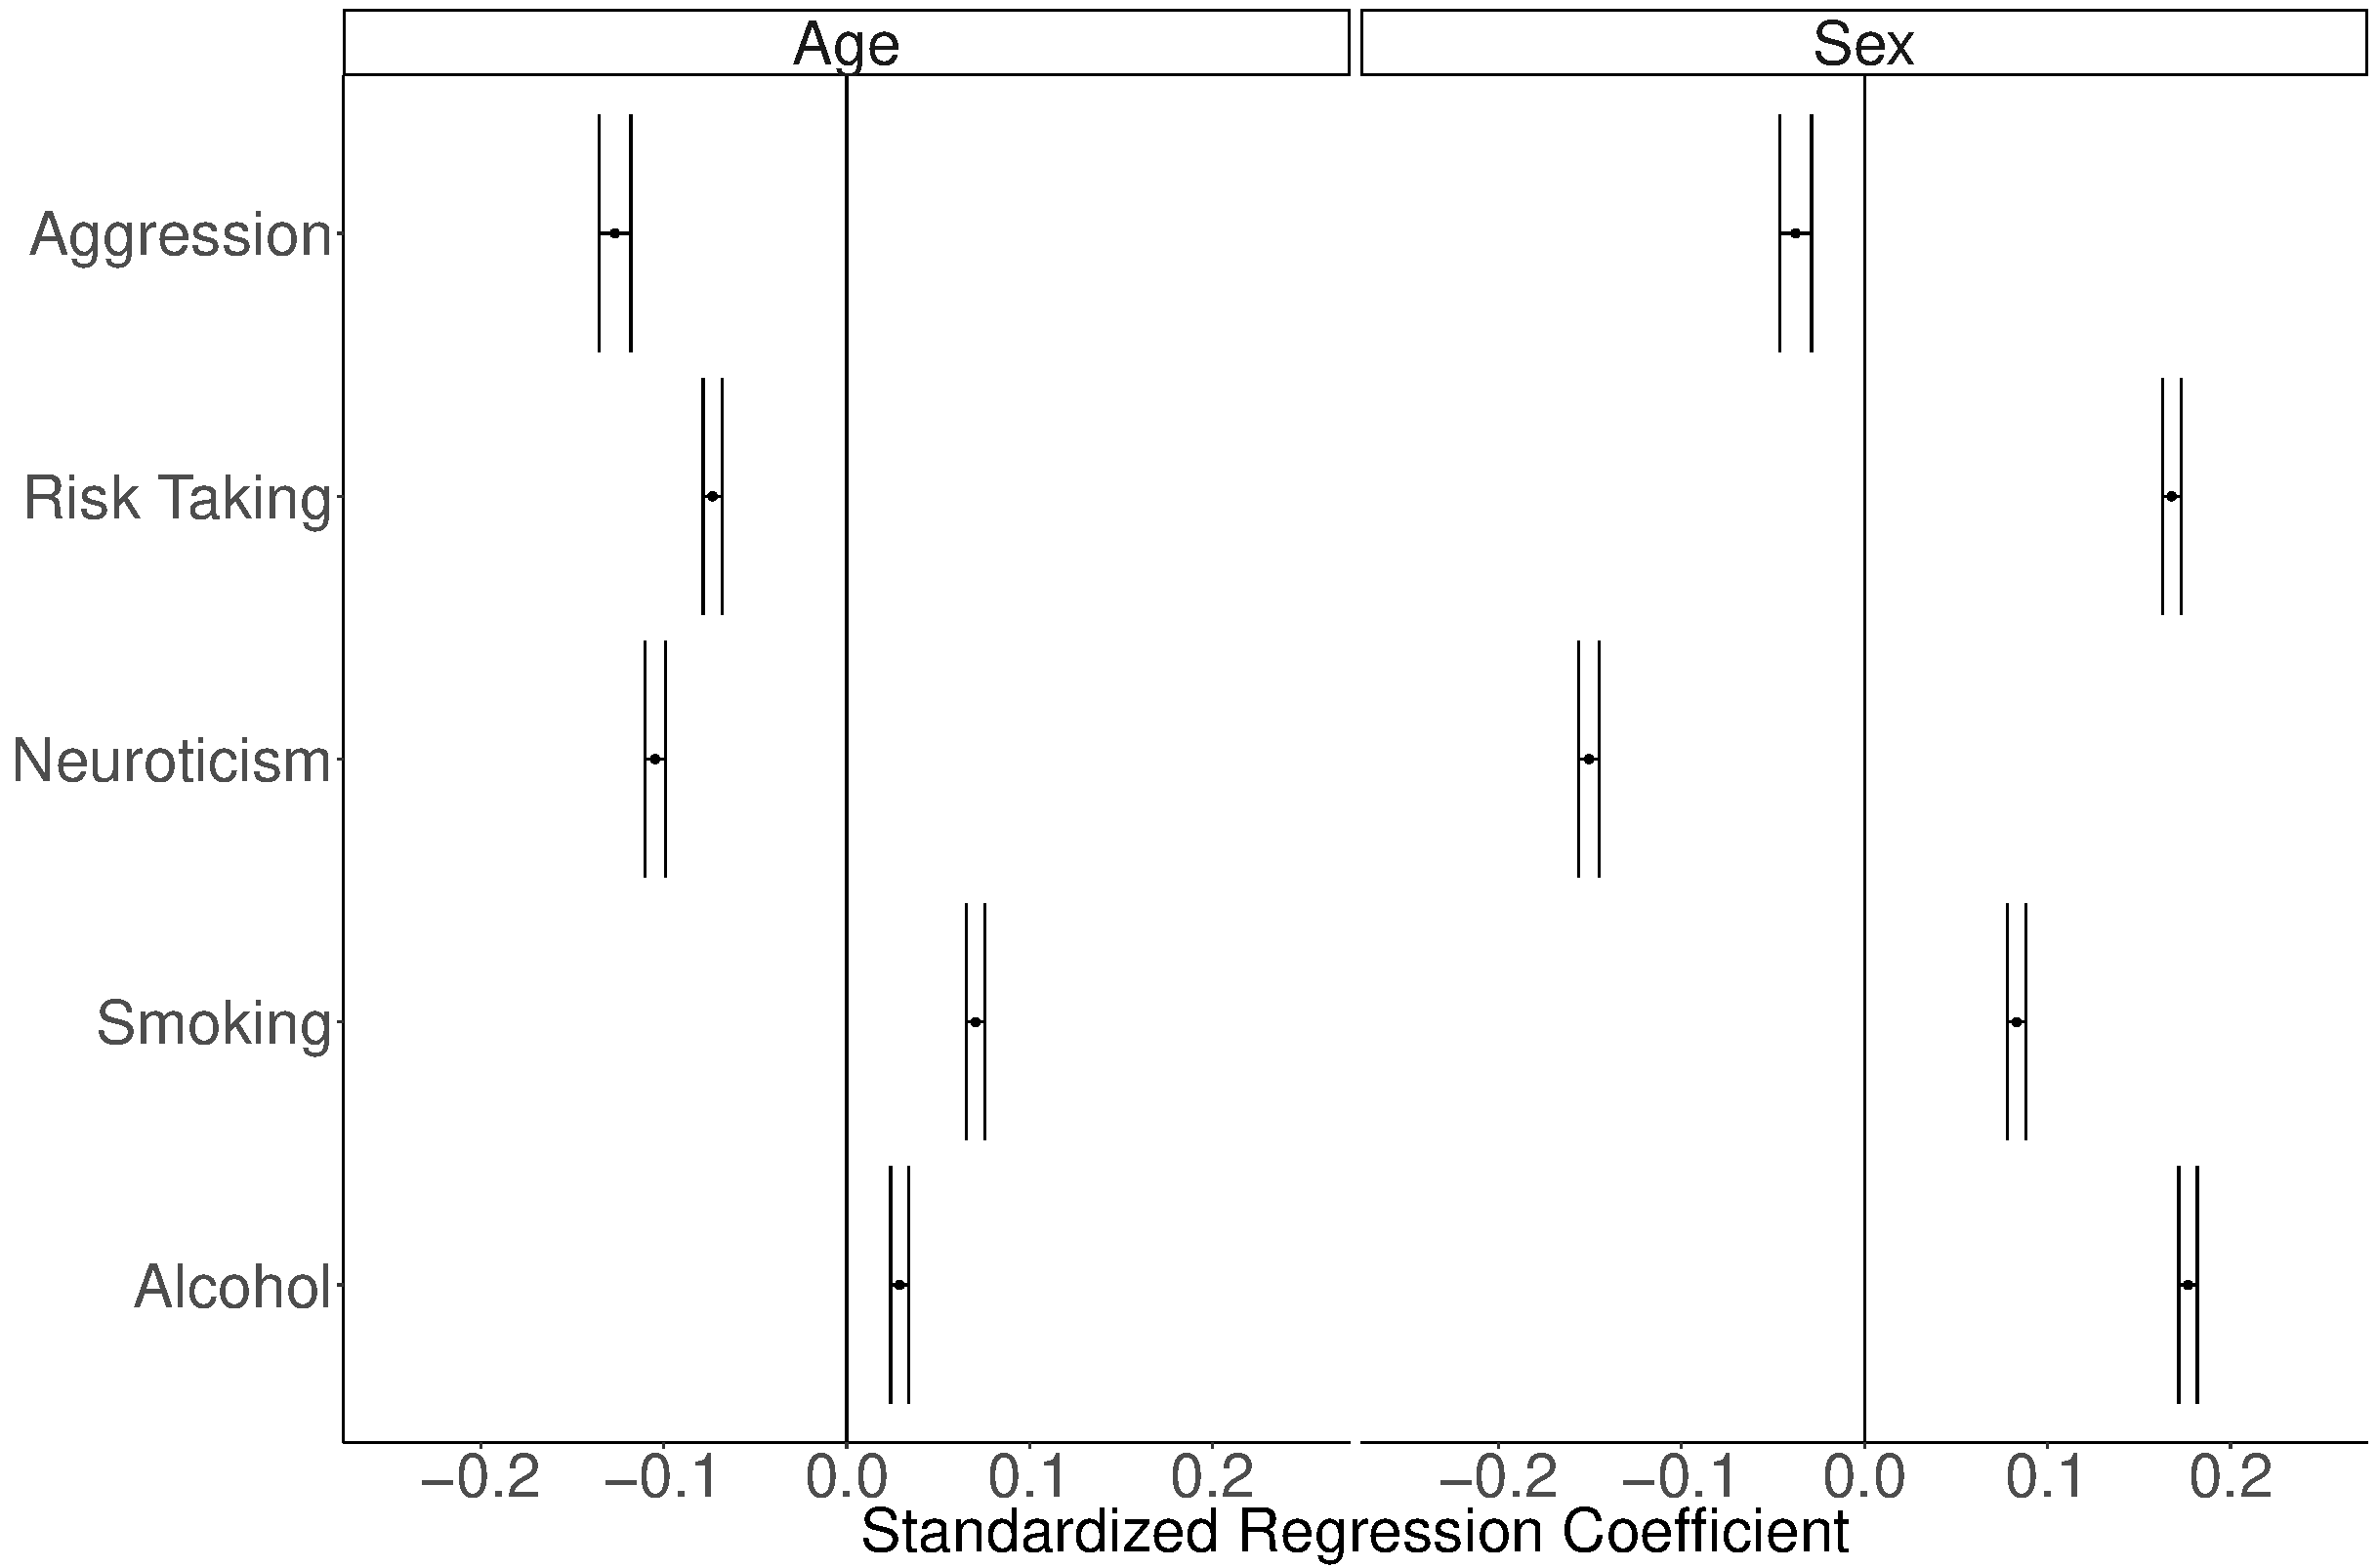
\includegraphics[width=0.8\linewidth]{ukb_assoc/figure/phenotype/descriptives_plots.pdf}
  \caption[Descriptive Statistics of Primary and Secondary Phenotypes]{
    Descriptive Statistics of primary and secondary phenotypes for all participants.
    (A) Standardized effect of sex (male, female) on phenotypes. 
    A positive effect size indicates greater prevalence in male than in female.
    Errorbars indicate the 95\% confidence interval.
    (B) Standardized effect of age on phenotypes.
    Errorbars indicate the 95\% confidence interval.
    (C) Barplot of neuroticism.
    The plot displays the frequency of each neuroticism score.
    (D) Barplot of alcohol intake.
    The plot displays the frequency of each alcohol intake score.
  }\label{fig:disc}
\end{figure}

\subsection{Phenotypic Correlations}
\label{sub:phenotype_correlations}

Phenotypic correlations are displayed in Figure~\ref{fig:corr_pheno}. 
All correlations were significant at $p\leq 0.05$ after adjusting for multiple testing using the Bonferroni correction.
Correlations between risk taking and impulsive aggression were $r(48540)=0.09 (p=3.25\times 10^{-85})$ relatively small
and I was unable to detect larger effects between impulsive aggression and alcohol consumption ($r(50220)=-0.05, p=2.20\times 10^{-28}$)
as well as smoking ($r(50106)=0.1, p=1.93\times 10^{-101}$).
Similar, risk taking displays only small correlations between
smoking ($r(146051)=0.09, p=4.07\times 10^{-260}$),
alcohol consumption ($r(146350)=0.06, p=3.25\times 10^{-85}$)
and neuroticism ($r(120201)=-0.03, p=1.56\times 10^{-32}$). 
Nevertheless, medium correlations were present between impulsive aggression and neuroticism ($r(41420)=0.33, p=0$).

\begin{figure}[htpb]
  \centering
  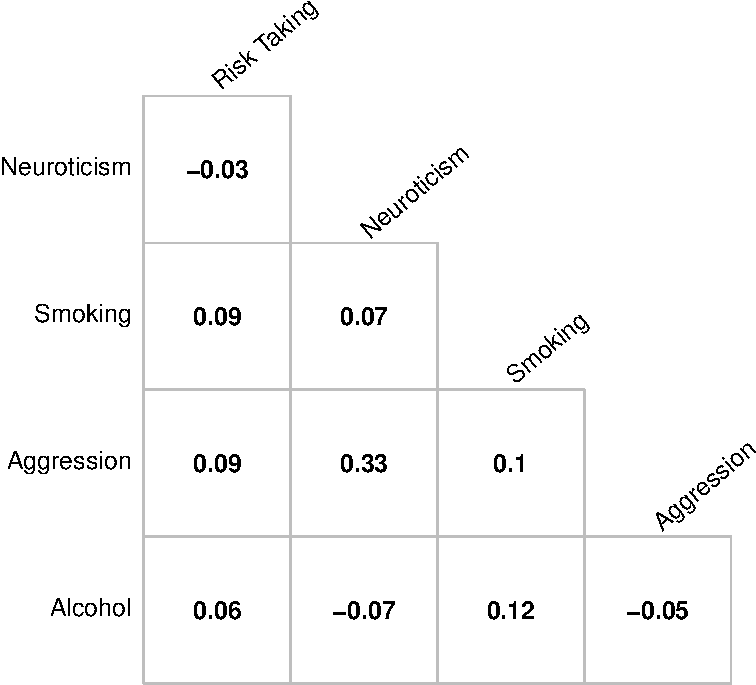
\includegraphics[width=0.6\linewidth]{ukb_assoc/figure/phenotype/corr_plot_ci.pdf} 
  \caption[Phenotypical correlations]{
    Phenotypical correlations among analyzed phenotypes for all subjects.
    Displayed correlations were all significant after adjusting for multiple testing using the Bonferroni correction.
    In contrast to the genetic correlations, Caucasian and non-Caucasian subjects were used.
  }\label{fig:corr_pheno}
\end{figure}

\subsection{GWAS of Impulsive Aggression and Risk Taking}
\label{sub:gwas}

Genome-wide association analysis reveled no genome-wide significant loci in $37,320$ impulsive aggression subjects (see Figure~\ref{fig:manhatten} panel A).
Observed SNP heritability was estimated at $5.32\% (SE=0.012)$ and is in line with previous estimated SNP heritabilities in behavioral traits.

The genome-wide association study on risk taking yielded two genome-wide significant loci in $120,286$ subjects on chromosome 3 and 6 (see Figure~\ref{fig:manhatten}, panel B).
Total observed SNP heritability is  $5.52\% (SE=0.0052)$, similar to that of impulsive aggression.
The ratio between the LD-score regression intercept $\beta_0$ and the mean of the $\chi^2$-test statistics ($(\beta_0 - 1)/(mean(\chi^2)-1)$),
which indicates the proportion of inflation due to factors other than polygenic heritability, is  negligible ($0.0422$, $SE=0.052$).
In addition, $\beta_0$ approaches 1 ($\beta_0=1.0082, SE=0.0056$) thus suggesting no population stratification (see Figure~\ref{fig:riskqq}).

\begin{figure}[!htpb]
  \begin{subfigure}{1\textwidth}
  \centering
  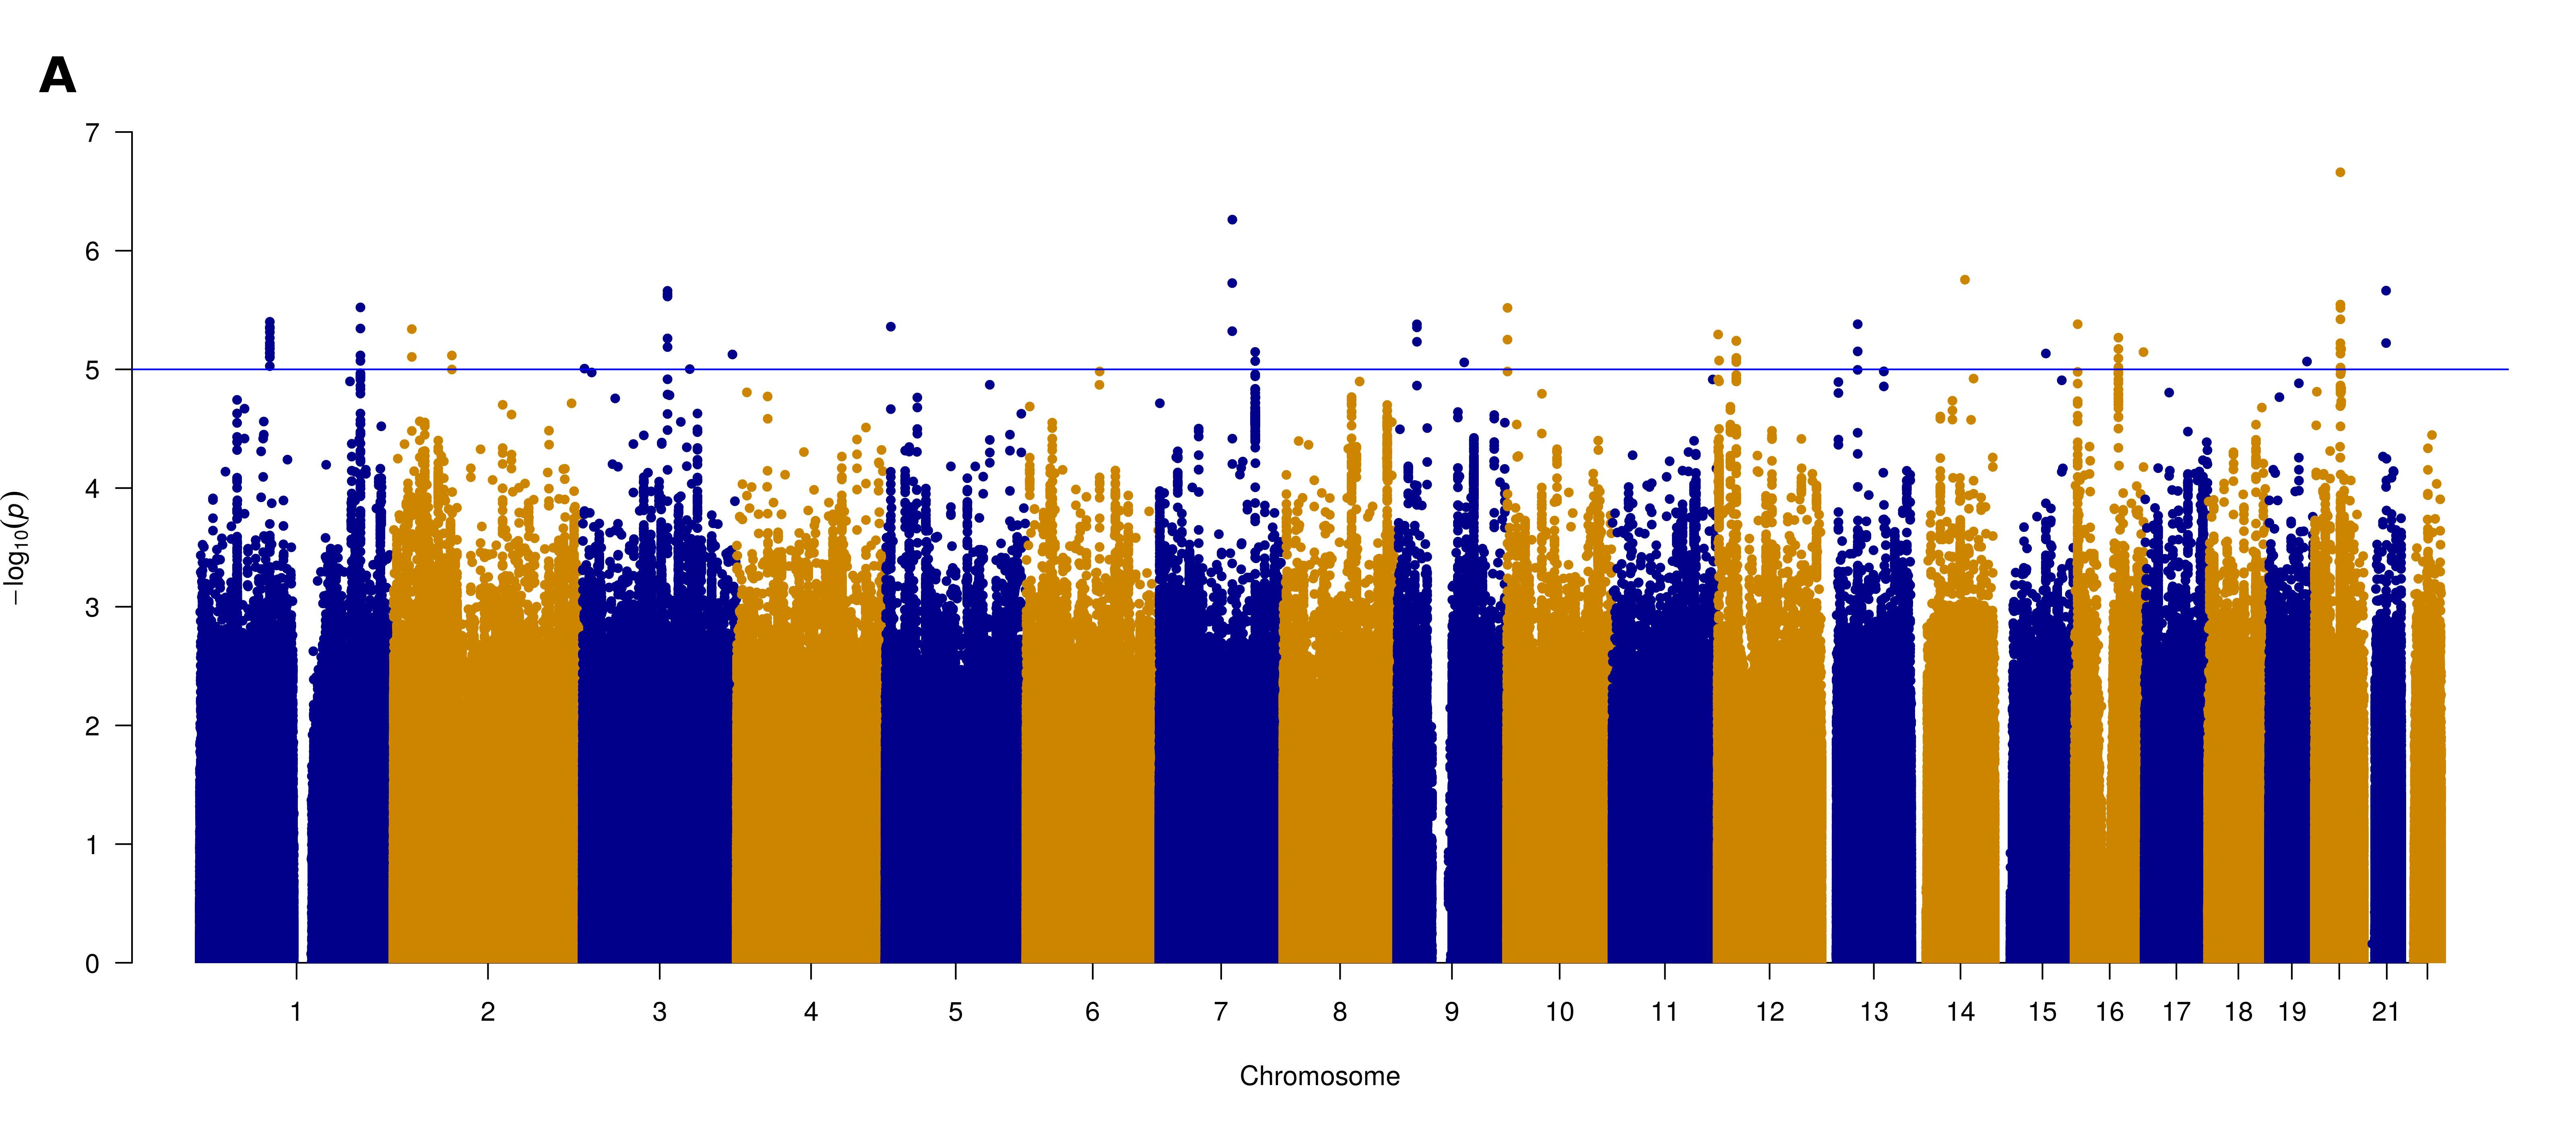
\includegraphics[width=0.8\linewidth]{ukb_assoc/figure/manhatten_plots/agg_manhatten_color_2_A.jpeg}
  \end{subfigure}
  \begin{subfigure}{1\textwidth}
  \centering
  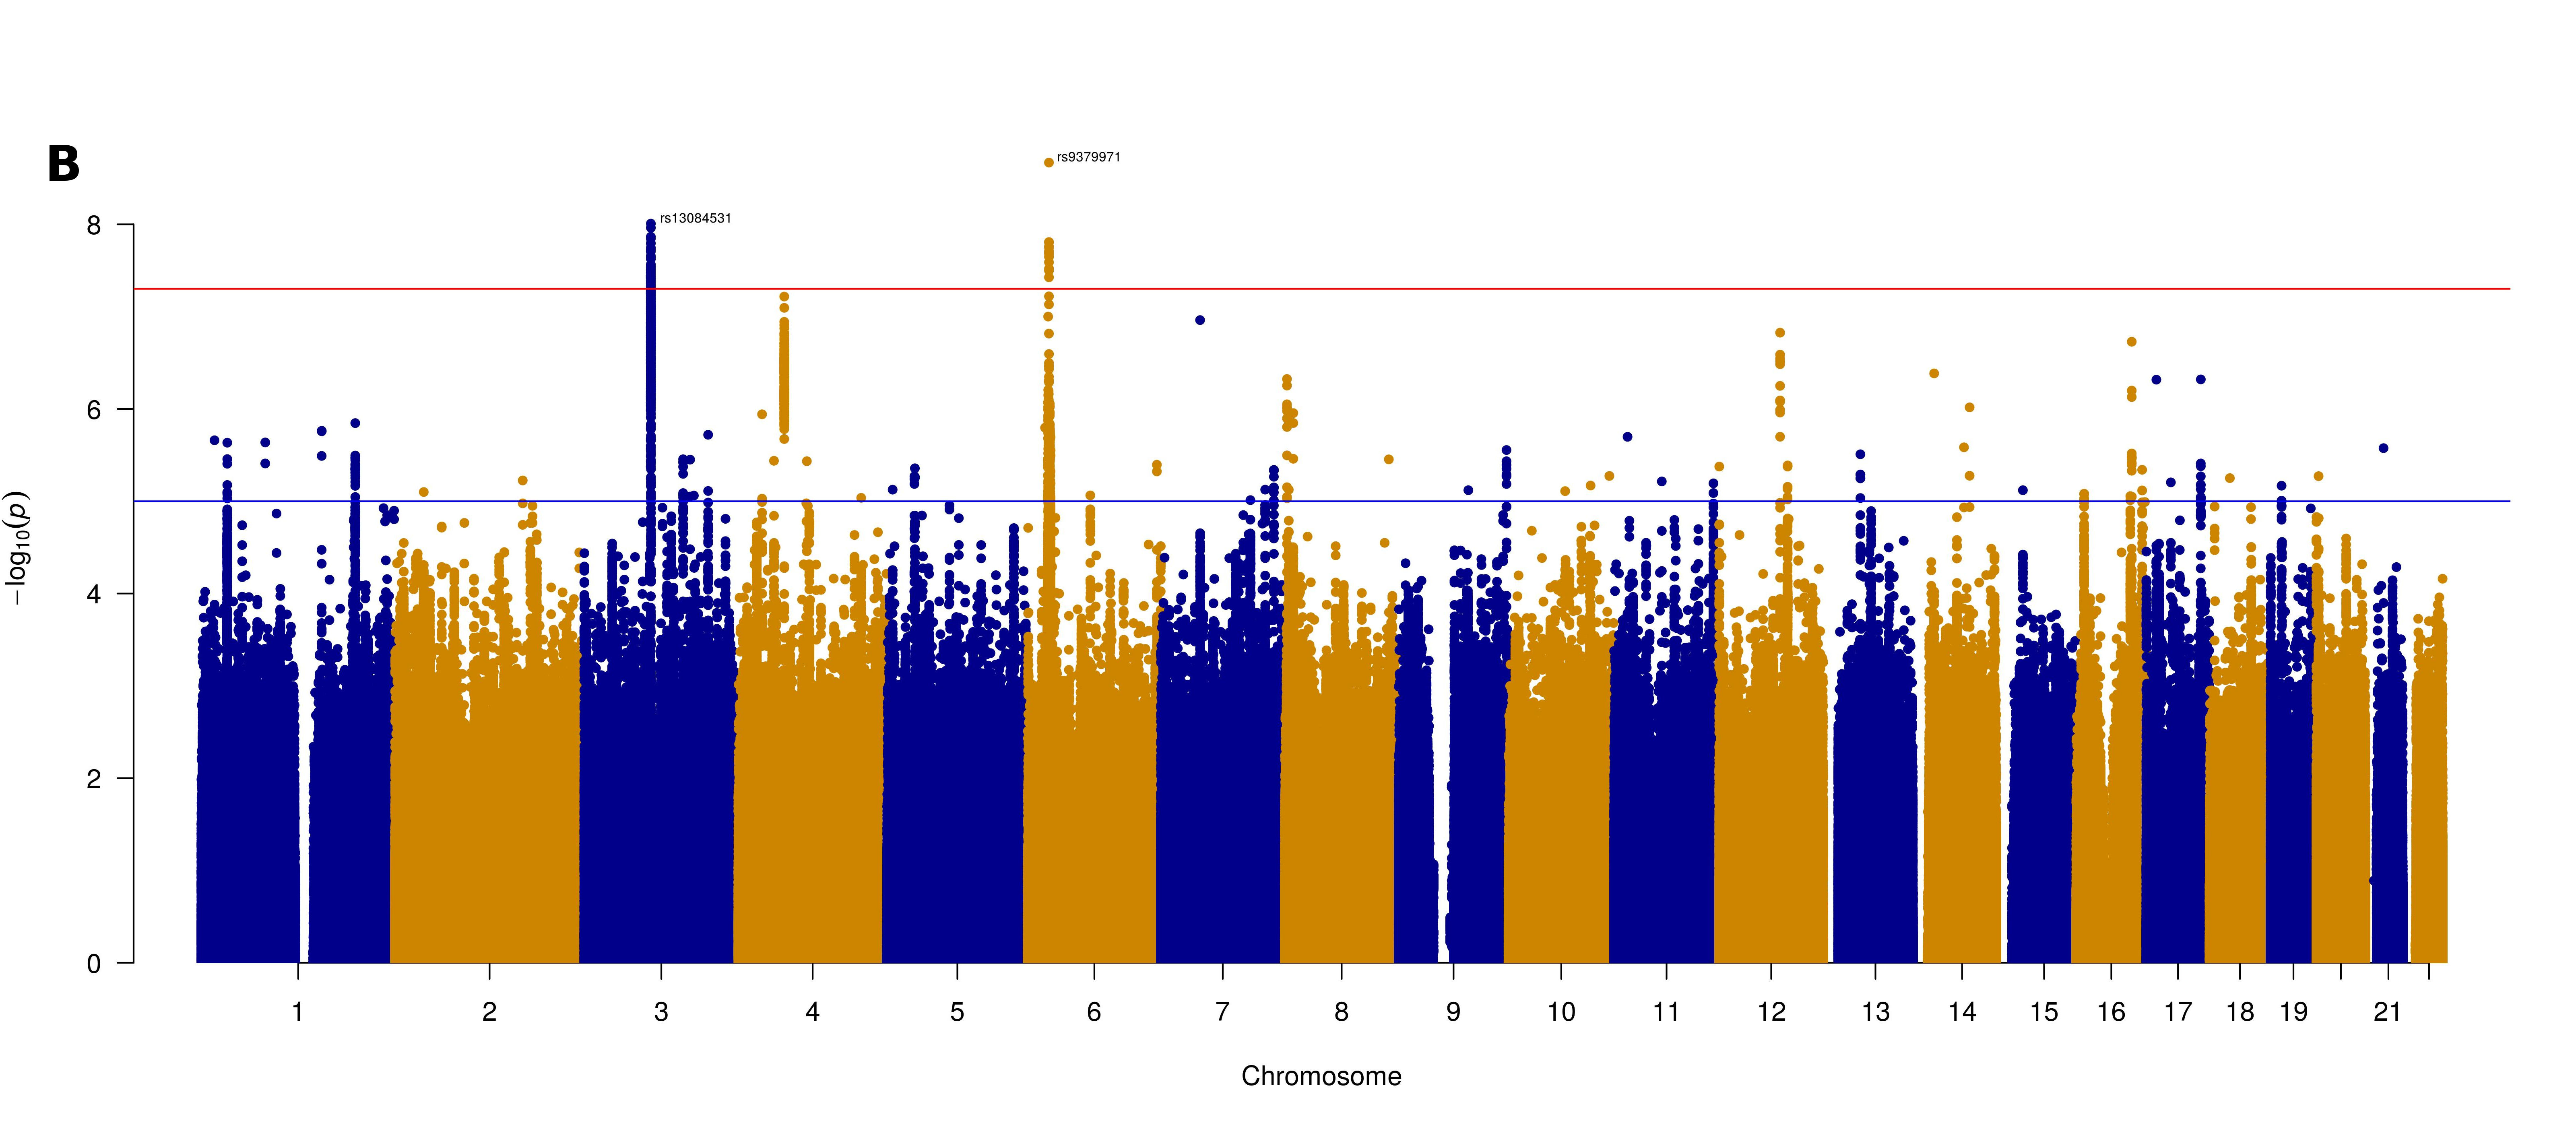
\includegraphics[width=0.8\linewidth]{ukb_assoc/figure/manhatten_plots/risk_manhatten_color_B.jpeg}
  \end{subfigure}
  \caption[Manhatten Plots]{
    Manhattan Plot for impulsive aggression (A)
    and risk taking (B).
    The red line in pannel B indicates genome wide significance level at $\alpha=5\times10^{-8}$.
    The blue line in panel A and B represents a suggestive genetic effect at $\alpha=5\times10^{-5}$.}\label{fig:manhatten}
\end{figure}

Closer inspection of the signal on chromosome 3 shows 2 lead SNPs namely \textit{rs1308431} and \textit{rs7639518} (see Table~\ref{tab:lead_snps_risk}).
However, \textit{rs1308431} and \textit{rs7639518} have different directions of effect.
Specifically, while the minor allele in \textit{rs76395182} is less common in affected ($0.330$) than unaffected individuals ($0.344$) the opposite is the case in \textit{rs13084531} ($0.233$ versus $0.222$).
The independence of these two signals was investigated using a conditional analysis.
Thus, genotypes at \textit{rs7639518} were regressed on the phenotype while adjusting for \textit{rs1308431}.
This conditional model indicates that \textit{rs7639518} is not independent of \textit{rs1308431} at a genome-wide level ($OR=0.957, t(107737)=-3.787, p=0.0001523$).

\paragraph{rs9379971}
\label{par:rs9379971}
This particular variant has the strongest association among all tested SNPs with a p-value of $2.14\times10^{-9}$ (see Figure~\ref{fig:rs9379971}). 
The SNP is an intronic variant and has not been associated with other phenotypes~\cite{Welter2014}.
The overall genomic region (6p22.5) has been associated with schizophrenia across multiple studies~\cite{Aberg2013,Shi2009}.

\paragraph{rs13084531}
\label{par:rs13084531}
This SNP has a comparable p-value ($9.826\times10^{-9}$) and is an intronic variant in very close proximity to the gene \textit{CADM2}.
The gene has been associated with BMI~\cite{Speliotes2010} as well as executive function and processing speed~\cite{Ibrahim-Verbaas2015}.
Interestingly, the SNP associated in the study by~\cite{Ibrahim-Verbaas2015} (\textit{rs17518584}) is in LD with \textit{rs13084531} ($r^2=0.4951;D'=0.9983$), suggesting a common locus for executive function and risk taking.
Specifically higher frequency of the risk allele in \textit{rs17518584} results in an increase in the number of risk allele in \textit{rs13084531}.
The corresponding genomic region (3p12.1) has been connected to spirometric measures in smokers~\cite{Lutz2015}.

\begin{table}
	\small
	\centering
	%latex.default(dat, title = "", file = paste0(outputfolder, "lead_snp_",     nameID, ".tex"), digits = 3, rowname = NULL, table.env = F)%
\begin{tabular}{rlrlrrrr}
\hline\hline
\multicolumn{1}{c}{CHR}&\multicolumn{1}{c}{SNP}&\multicolumn{1}{c}{BP}&\multicolumn{1}{c}{A1}&\multicolumn{1}{c}{N}&\multicolumn{1}{c}{OR}&\multicolumn{1}{c}{STAT}&\multicolumn{1}{c}{P}\tabularnewline
\hline
$3$ & rs13084531 & $85553994$ & G & $115264$ & $0.936$ & $5.73$ & $9.83e-09$\tabularnewline
$6$ & rs9379971  & $27259308$ & T & $109344$ & $1.065$ & $ 5.99$ & $2.14e-09$\tabularnewline
\hline
\end{tabular}

  \caption[Lead SNPs]{
    Lead SNPs reaching genome wide significance for risk-taking.
    SNPS are listed by chromosome (CHR) and position (BP).
    Odds ratios as well as test statistics of each SNP are indicated by OR and STAT correspondingly.
    P-values of each SNP are shown in the last column (P).
  }\label{tab:lead_snps_risk}
\end{table}

\subsection{Conditional FDR}
\label{sub:conditional_fdr}

Pleiotropy informed \acrfull{cfdr} was used to identify additional genetic loci associated with risk taking or impulsive aggression.
Figure~\ref{fig:cFDR} shows the conditional QQ plots for both aggression and risk taking for each of the chosen thresholds and conditional phenotypes.
An inflation within a conditional QQ plot can indicate pleiotropic effects.
Both aggression and risk taking, conditional on each other did not result in any noticeable pleiotropic effect.
However, risk taking was noticeably inflated conditional on SNPs which reached a relatively low $p$-value cut-off in neuroticism, alcohol consumption, and smoking.
Interestingly, inflation of risk taking SNPs conditional on neuroticism was not persistent across the chosen thresholds.
In particular, while considerable inflation could be observed at $p\leq0.1$, at lower p-value threshold this effect was reduced.
In contrary, the inflation observed when conditioning on alcohol consumption and smoking was persistent across the three thresholds.

As already indicated in Figure~\ref{fig:cFDR}, impulsive aggression conditional on the four remaining phenotypes did not result in any loci with an $cFDR\leq0.01$.
Nevertheless, cFDR identified a single independent loci, \textit{rs570682061}, in risk taking which passes both $cFDR\leq0.01$ as well replication in an independent sample after clumping (Table~\ref{tab:cFDR}).
However, closer inspection shows that the loci \textit{rs570682061} is in high LD with \textit{rs13084531} ($r^2=0.4946;D'=1$).

\begin{figure}[!htpb]
  \centering
	\begin{subfigure}{1\textwidth}
		\centering
    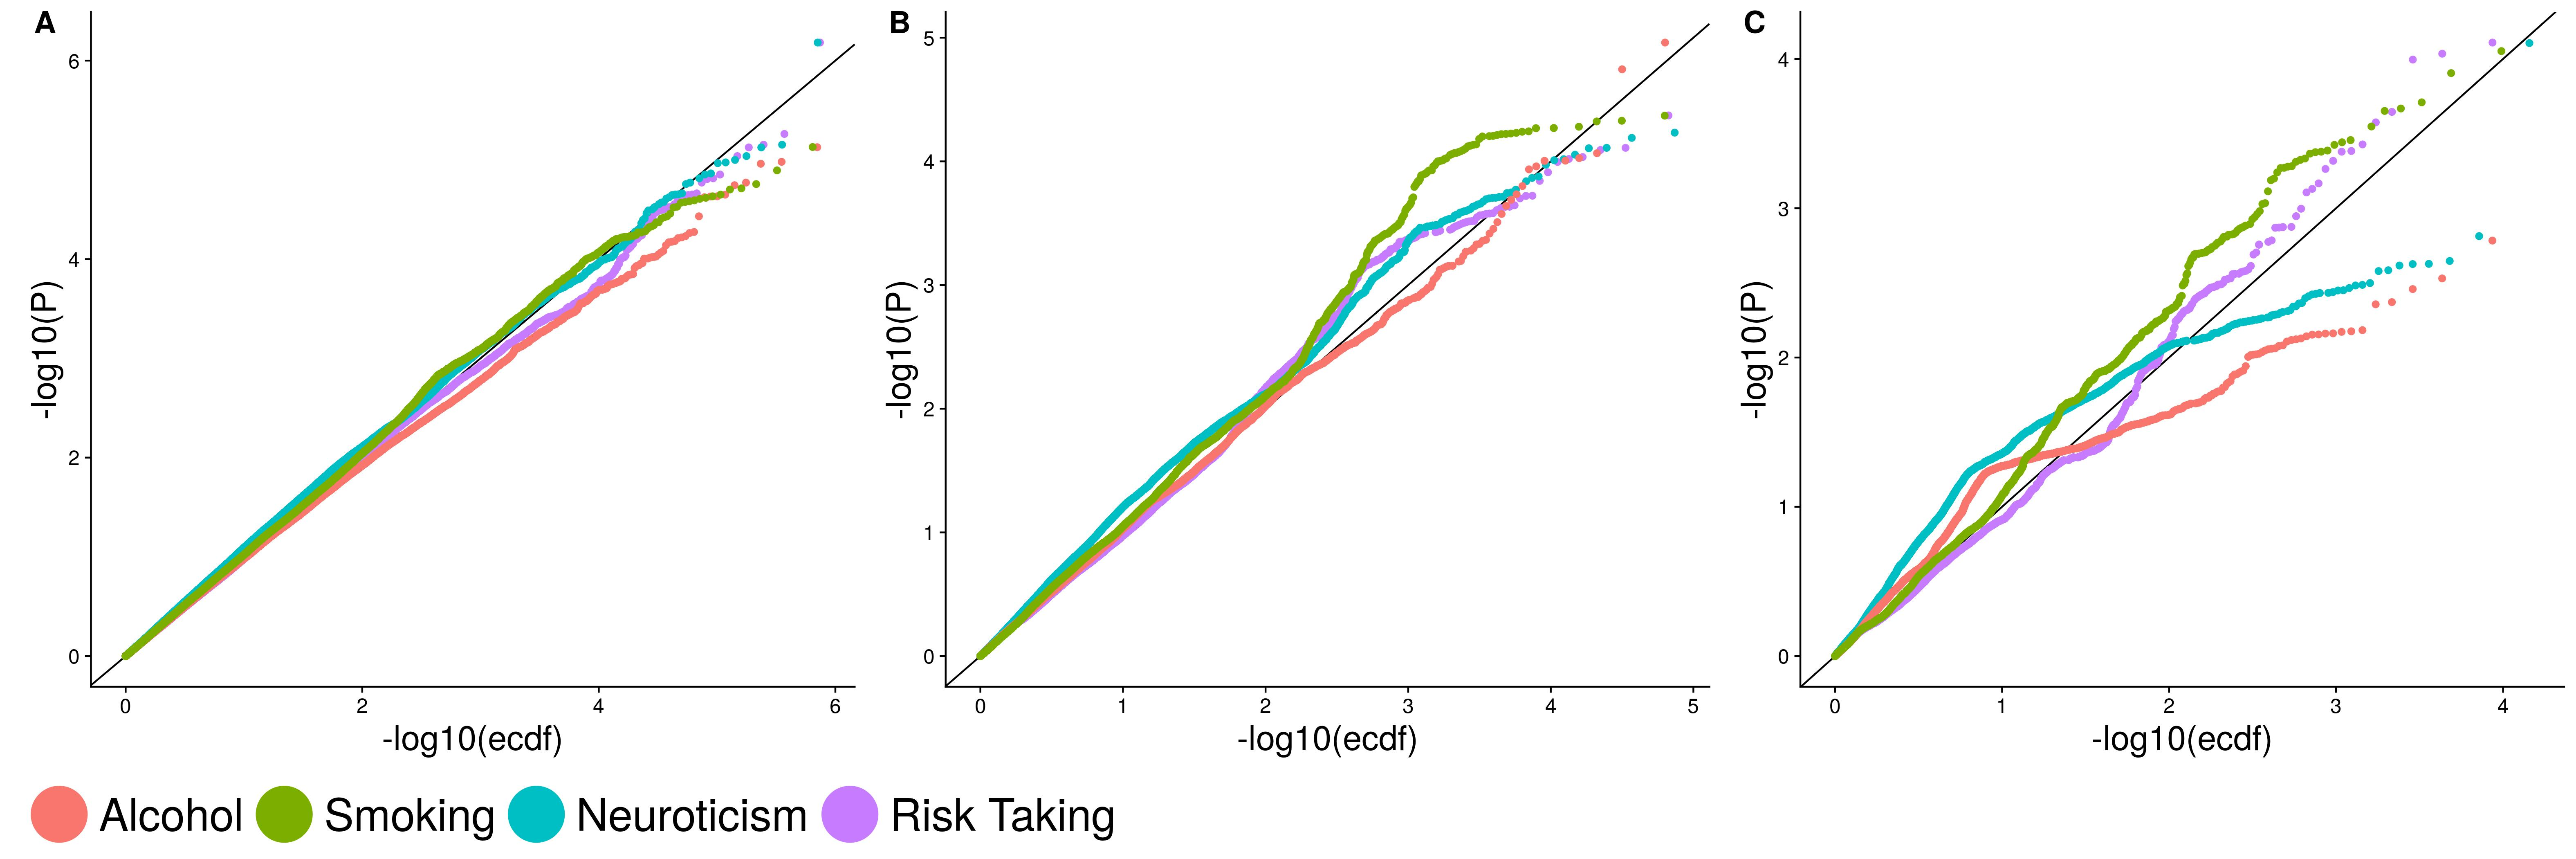
\includegraphics[width=1\linewidth]{ukb_assoc/figure/cFDR/agg_cond.jpeg}
	\end{subfigure}
	\begin{subfigure}{1\textwidth}
		\centering
    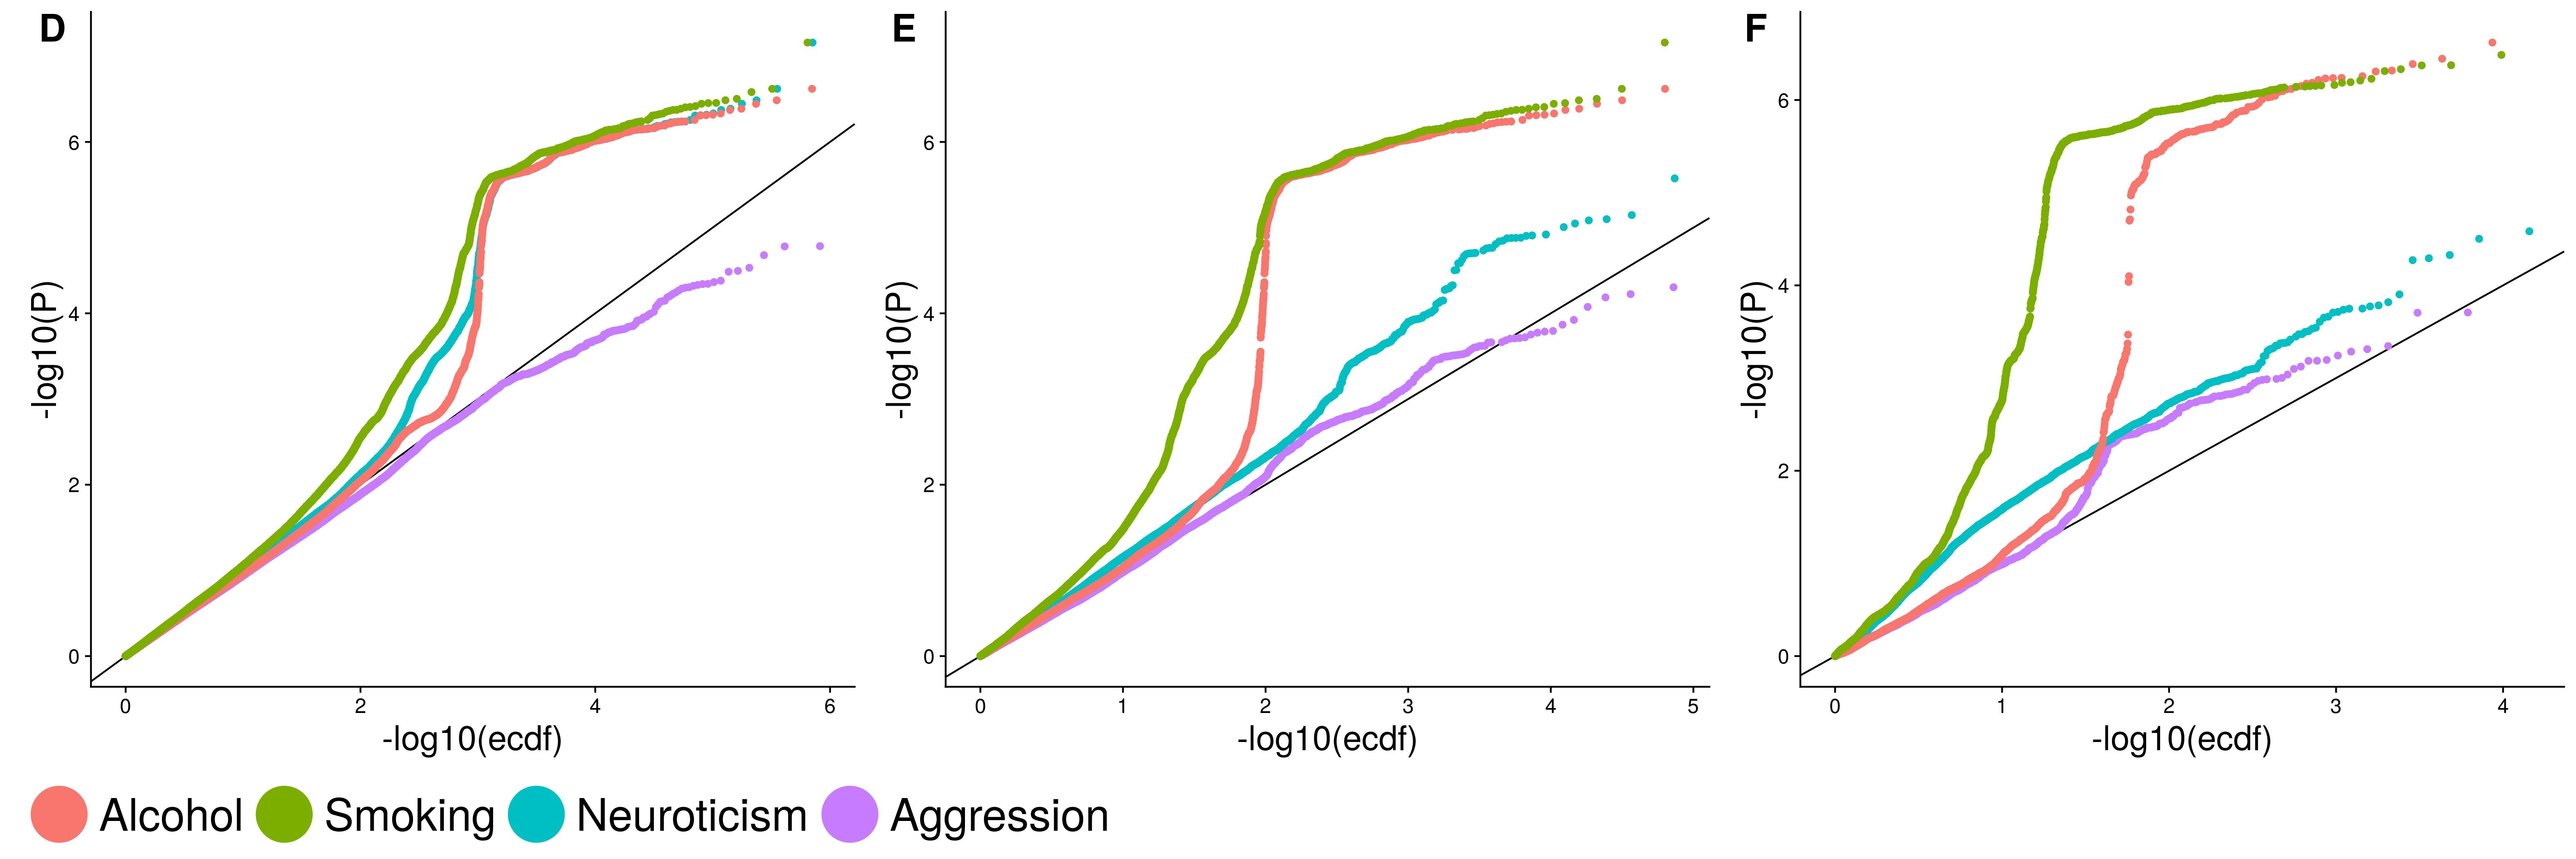
\includegraphics[width=1\linewidth]{ukb_assoc/figure/cFDR/risk_cond.jpeg}
	\end{subfigure}
  \caption[Conditional QQ plots]{
    Conditional QQ plots for both risk taking and aggression. 
    Panels A--C present the  QQ-plots for impulsive aggression,
    conditional on the remaining phenotypes given threshold $p\leq0.1$, $p\leq0.01$, $p\leq0.001$ respectively.
    Similarly, panels D--F are the  QQ-plots for risk taking, conditional on the remaining phenotypes across the three thresholds.\label{fig:cFDR}}
\end{figure}


\begin{table}[htpb]
  %latex.default(dat, title = "", file = "risk_cFDR.tex", cellTexCmds = cell.format,     numeric.dollar = FALSE, digits = 3, rowname = NULL, table.env = F)%
\begin{center}
\begin{tabular}{rlrrlllr}
\hline\hline
\multicolumn{1}{c}{CHR}&\multicolumn{1}{c}{SNP}&\multicolumn{1}{c}{cFDR}&\multicolumn{1}{c}{Z}&\multicolumn{1}{c}{A1}&\multicolumn{1}{c}{A2}&\multicolumn{1}{c}{$\delta$}&\multicolumn{1}{c}{$Z_{\delta}$}\tabularnewline
\hline
    1&   rs1912231&   5.25e-03&    4.34&   C&   T&   Alcohol&    3.62\tabularnewline
    3&   rs9870448&   2.77e-04&   -5.24&   A&   G&   Alcohol&   -3.89\tabularnewline
\bfseries    3&\bfseries   rs570682061&\bfseries   6.64e-05&\bfseries    5.22&\bfseries   A&\bfseries   AT&\bfseries   Smoking&\bfseries    3.67\tabularnewline
    6&   rs7744605&   7.52e-05&    5.16&   C&   A&   Smoking&    3.27\tabularnewline
    6&   rs9468372&   2.06e-04&    4.88&   T&   A&   Smoking&    3.42\tabularnewline
    8&   rs1968400&   9.86e-03&    3.67&   G&   C&   Smoking&    3.23\tabularnewline
    8&   rs116807689&   2.62e-03&    4.16&   A&   G&   Smoking&    3.73\tabularnewline
   10&   rs67657945&   2.13e-03&   -4.23&   CT&   C&   Smoking&   -3.21\tabularnewline
\hline
\end{tabular}\end{center}

  \caption[Conditonal Analysis]{
    Independent loci ($r^2 < 0.05$) with $cFDR\leq0.01$.
    SNPs are listed by location (CHR) and conditional phenotype ($\delta$).
    Z-scores are indicated for both risk taking and the conditional phenotype.
    Data were adjusted for genomic inflation.
    SNPs in bold indicate replication in an independent sample.
  }\label{tab:cFDR}
\end{table}

\subsection{Genetic Correlations}
\label{sub:genetic_correlations_internal}

Figure~\ref{fig:gcor} displays the genetic correlations of analysed phenotypes.
The largest genetic correlations could be observed between impulsive aggression and neuroticism ($r_g=0.63, SE=0.083, p=4.64\times 10^{-14}$), 
followed by a considerable correlation between risk taking and aggression ($r_g=0.44, SE=0.103, p=2.66\times 10^{-5}$).
Interestingly, relatively large negative correlations are also present between alcohol consumption and aggression ($r_g=-0.39, SE=0.0892, p=1.69\times 10^{-5}$)
as well as between smoking and aggression ($r_g=0.4, SE=0.071, p=1.64\times 10^{-08}$).
Correlation, between smoking and alcohol consumption was not significant as well of neglectable effect ($r_g=0.06, SE=0.044, p=0.155$).
Interestingly, these respectively high genetic correlations are not reflected in the corresponding conditional FDR (see Figure~\ref{fig:cFDR}).

Furthermore, risk taking shows non-significant and small correlation with neuroticism ($r_g=-0.12, SE=0.0738, p=0.106$) and
alcohol consumption ($r_g=0.07, SE=0.051, p=0.196$) but the correlation between risk taking and smoking ($r_g=0.34, SE=0.051, p=2.40\times 10^{-11}$) is considerable.
In addition, medium correlations were present between neuroticism and alcohol consumption ($r_g=-0.17, SE=0.040, p=2.63\times 10^{-4}$). 
Effects were also present between neuroticism and smoking, but did not pass multiple testing ($r_g=0.16, SE=0.066, p=0.017$).

\begin{figure}[!h]
	\centering
  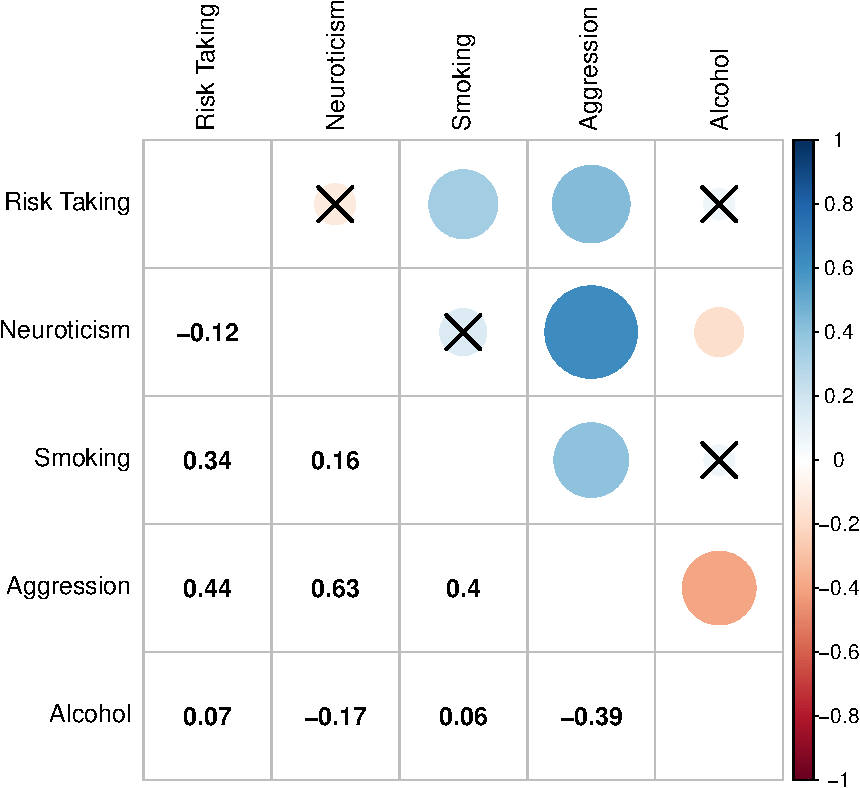
\includegraphics[width=0.8\linewidth]{ukb_assoc/figure/genetic_corr/gcorr_plot_circle_full_se.pdf}
  \caption[Genetic Correlations]{Genetic Correlations.
    Pairwise genetic correlations across analysed phenotypes.
    The lower triangular matrix presents the numeric correlations, while the upper part is a visual representation of the strengths and direction of the correlations.
    A cross indicates a non-significant correlation after adjusting for multiple testing.
  }\label{fig:gcor}
\end{figure}
